%% A simple template for a scientific article using the Hagenberg setup
%% based on the standard LaTeX 'article' class
%%% äöüÄÖÜß  <-- no German umlauts here? Use a UTF-8 compatible editor!

%%% Magic comments for setting the correct parameters in compatible IDEs
% !TeX encoding = utf8
% !TeX program = pdflatex 
% !TeX spellcheck = en_US
% !BIB program = biber

\RequirePackage[utf8]{inputenc} % Remove when using lualatex or xelatex!
\RequirePackage{hgbpdfa}        % Creates a PDF/A-2b compliant document

\documentclass[english,smartquotes]{hgbarticle}
%\documentclass[english,twocolumn, smartquotes]{hgbarticle}
% Valid options in [..]: 
%    Main language: 'german' (default), 'english'
%    Turn on smart quote handling: 'smartquotes'
%    APA bibliography style: 'apa'
%    Typeset the text in two columns: 'twocolumn'
%%%-----------------------------------------------------------------------------

\usepackage{lipsum}       % Create lorem ipsum dummy text (can be removed)
\usepackage{hyperref} % clickable www links
\hypersetup{
colorlinks=true,
linkcolor=blue,
urlcolor=magenta,
}
\flushbottom              % Add vertical space where necessary to fill the page
\graphicspath{{images/}}  % Location of images and graphics
\bibliography{references} % Biblatex bibliography file (references.bib)

% for unside down text
\usepackage[framemethod=tikz]{mdframed}
\newtheorem{question}{Puzzle}
\mdfdefinestyle{que}{
  linecolor=cyan,
  backgroundcolor=cyan!20,
}
\surroundwithmdframed[style=que]{question}
\newtheorem{answer}{}
\mdfdefinestyle{ans}{
  linecolor=cyan,
  backgroundcolor=yellow!20
}
\surroundwithmdframed[style=ans]{answer}
\usepackage{environ}
\NewEnviron{rotanswer}{%
  \begin{tikzpicture}
  \node[rotate=180,inner sep=0pt] {\parbox{\linewidth}{%
  \begin{answer}
  \BODY
  \end{answer}}};
\end{tikzpicture}%
}
% for unside down text https://tex.stackexchange.com/a/161886/64425
%%%-----------------------------------------------------------------------------
\begin{document}
%%%-----------------------------------------------------------------------------

\author{
	Kedar Mhaswade\\ 
	\email{kedar.mhaswade@gmail.com}
}
\title{A Social Media Combinatorial Problem}
\date{}

%%%-----------------------------------------------------------------------------
\maketitle
%%%-----------------------------------------------------------------------------

\begin{abstract}\noindent
This article discusses an algorithmic approach and a computer program based on it
to solve an elementary combinatorial problem popular on social media.
\end{abstract}

%%%-----------------------------------------------------------------------------

\section{Introduction}

Consider the following puzzle\footnote{I first heard it from \href{https://sunilsingh-42118.medium.com/}{Sunil Singh}, a mathematics educator}:

\begin{question}
How can you make $24$ using the numbers $1, 3, 4,$ and $6$ exactly once each, and the four arithmetic operations ($+, -, \times, \div$) any number of times\footnote{Using a number formed by concatenating two or more numbers (e.g. $13$) is disallowed}?
\end{question}

A ready-made answer is probably just an Internet search away. Just for fun, however, one should find such an arithmetic expression without searching it on the Web. The author took quite some time to find it.

\subsection{Initial Impressions}
This puzzle is surprisingly challenging, especially if one is not well-versed with solving such puzzles. We take arithmetic for granted, but the four basic operations combine with four small numbers to render this puzzle tantalizingly difficult. This is so even if you could somehow solve it.

In our attempts, we may start with some heuristics: If we can make an expression using 1, 3, and 4 that evaluates to 4, then we can make 24 by multiplying it by 6. We have a different puzzle now, which is just as tricky.

We may try parenthesizing parts of shorter expressions (e.g. $((6+4)-1)\times3 = 27$). After toiling for a while we might \textit{luckily} find the magic expression.

But we may not. What if no such expression exists? Can we tell if one exists at all? If more than one solution exist, can we find them all? Can we even tell if we have examined \textit{all} expressions possible?

We keep \textit{feeling} inadequate as we continue searching \dots
\section{An Algorithmic Approach to Searching}
As you keep searching, you may feel frustrated. After all, what we are do is form expressions of four numbers and four familiar arithmetic signs and evaluate it on the fly. It gets quite mechanical and hence boring after a short while. But we tend not to give up for a perceived shame grips us. After all, we have been seeing $+, -, \times, \div$ since first grade!

Even after eventually finding the expression, we keep wondering if we weren't lucky. In case we are about to abandon the search, we seem to lack the confidence that we have indeed examined every expression. 

Maybe we have picked up some prejudices in our childhood and carried them along unknowingly. Perhaps we should develop a different perspective. But, most of all, we feel the need of an assistance from a machine that carries out the calculations, well, mechanically. It's a solace that just such an accomplice exists: A computer! 

A computer is astoundingly fast at performing known calculations precisely and, at the same time, thankfully dumb at showing any originality (even when there is a tremendous pressure of Artificial Intelligence techniques of the modern times) in devising \textit{abstractions}, the indomitable spirit of computing.

\subsection{An Insight}
\subsection{The Algorithm}
\subsection{An Implementation}
\section{Summary and Conclusion}

\section{Answer to the Puzzle}
\begin{rotanswer}
$6\div(1-(3\div 4))$
\end{rotanswer}

%
\begin{equation}
\bar{\mathbf{M}} =  
\begin{pmatrix}
	A \ast H^{G}_{\sigma}   & C \ast H^{G}_{\sigma} \\
	C \ast H^{G}_{\sigma}   & B \ast H^{G}_{\sigma} 
\end{pmatrix}
=
\begin{pmatrix}
	\bar{A}   & \bar{C} \\
	\bar{C}   & \bar{B} 
\end{pmatrix}
\end{equation}
%
may fit without any modification, larger structures like the one shown in
Equation \ref{wideEquation} need special treatment.
%
\begin{figure*}[t]
	\begin{equation}
		\begin{split}
			\lambda_{1,2}
			&= \frac{\mathrm{tr}(\bar{\mathbf{M}})}{2} \pm \sqrt{\Bigl
			(\frac{\mathrm{tr}(\bar{\mathbf{M}})}{2}\Bigr)^2
			- \mathrm{det}(\bar{\mathbf{M}})}  \\
			&= \frac{1}{2} \cdot \left( \bar{A} + \bar{B} \pm \sqrt{\bar{A}^2 -
			2 \cdot \bar{A} \cdot \bar{B} + \bar{B}^2 + 4 \cdot \bar{C}^2}
			\right)
			,
		\end{split}
		\label{wideEquation}
	\end{equation}
\end{figure*}
%
In this case, the equation was wrapped into a \verb!\begin{figure*}! \ldots
\verb!\end{figure*}! environment, which produces an unnumbered float object
that extends across the full page width. Additional details can be found in
the source text.

\subsection{Graphics and Images}

Similarly, the horizontal space available for graphical elements is the width
of a single column. Thus elements inserted with \verb!\includegraphics{..}! 
should use the length \verb!\columnwidth! for scaling. An example is shown in
Fig.~\ref{fig:CocaCola} (see the source text for details).

\begin{figure}
	\centering
	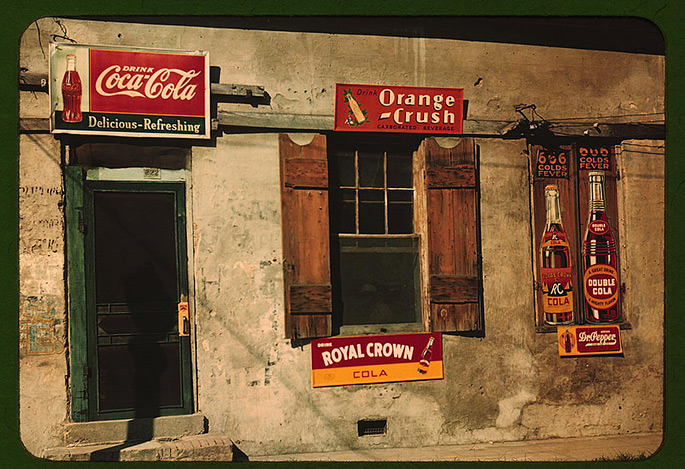
\includegraphics[width=1.0\columnwidth]{cola-public-domain-photo-p}
	\caption{Coca-Cola advertisement photographed in 1940 \cite{CocaCola1940}.}
	\label{fig:CocaCola}
\end{figure}

And by the way, the \texttt{lipsum} package was used to create the following
dummy texts. 

\subsection{Bibliography}

The use of citations and the compilation of the bibliography work much the
same as in the thesis template. The only difference is that
\verb!\printbibliography! is used directly at the end of the document.

%%%-----------------------------------------------------------------------------

\section{Existing Techniques}

\lipsum[2-4]

%%%-----------------------------------------------------------------------------

\section{Our Radically New Approach}

\lipsum[5-7]

%%%-----------------------------------------------------------------------------


%%%-----------------------------------------------------------------------------
\printbibliography % alternatively: \MakeBibliography[nosplit]
%%%-----------------------------------------------------------------------------

%%%-----------------------------------------------------------------------------
\end{document}
%%%-----------------------------------------------------------------------------
